\chapter{Erkundeter Beruf}

\section{ALlgemeines}

    Ich habe den Beruf des Anwendungsentwicklers mit Schwerpunkt auf Java-Development kennengelernt. Bei KIS sind ca. 100 Anwendungsentwickler angestellt. Um den Beruf des Anwendungsentwicklers zu erlernen ist i. d. R. ein Studium der angewandten Informatik von Nöten. Dieses kann entweder an einer Universität oder einer dualen Hochschule absolviert werden. Die Regelstudienzeit beträgt jeweils 6 Semester. 

\section{Arbeitsweise}

    \begin{figure}[H]
        \centering
        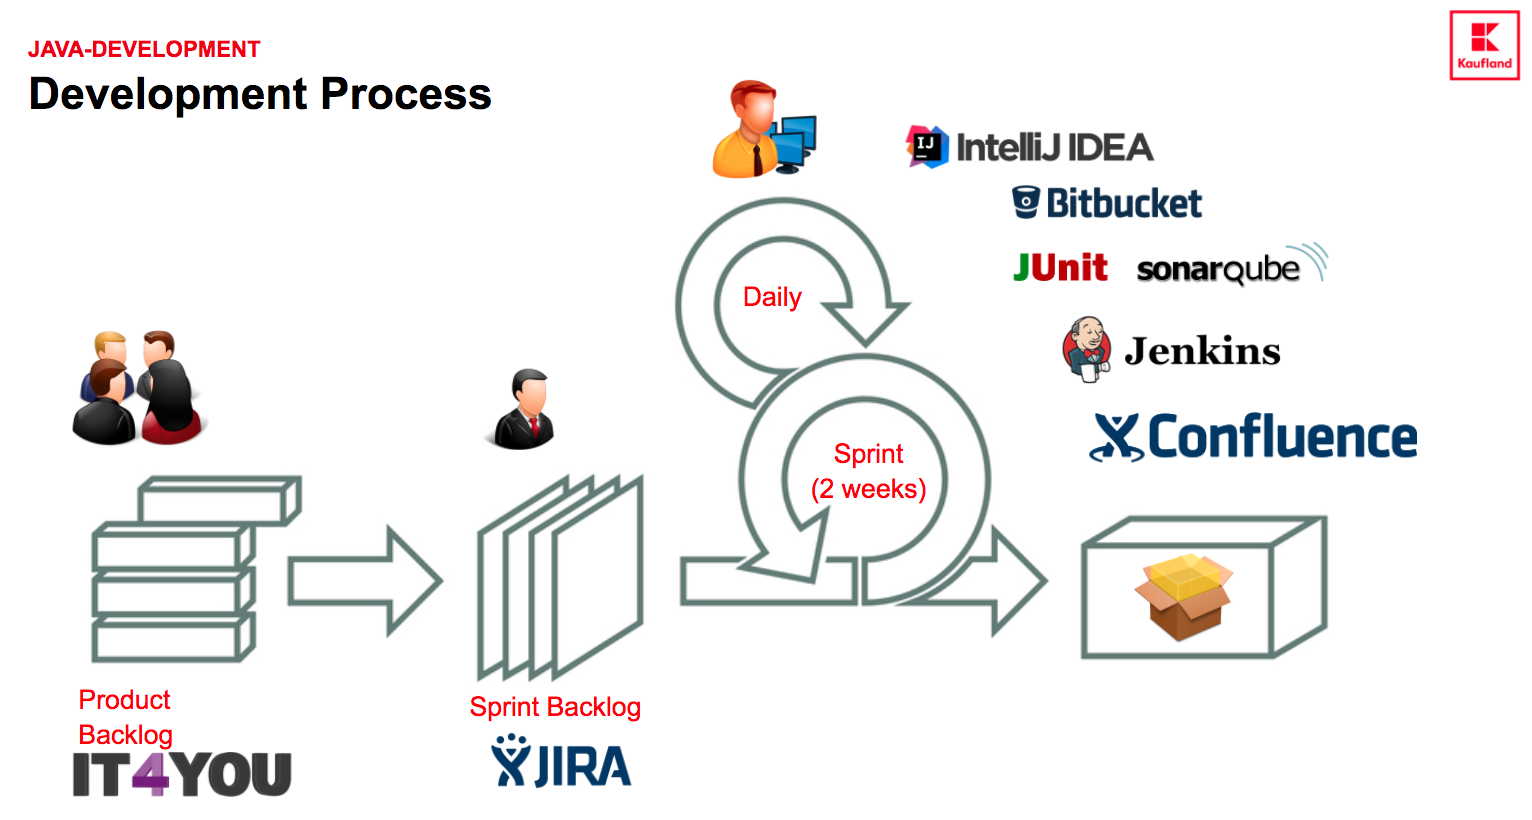
\includegraphics[width=\textwidth]{include/images/DevelopmentProcess.png}
        \caption{Entwicklungsprozess Scrum}
        \small Der bei der AE weit verbreitete Entwicklungsprozess wird auch bei Kaufland verwendet. Am Rand des Schuabildes sind die bei den jeweiligen Arbeitsschritten bei Kaufland verwendeten Werkzeuge bebildert.
        \label{fig-Development-Process}
    \end{figure}

    Der Entwicklungsprozess startet mit einer Idee aus dem FB (Produkt Backlog). Durch Beratung mit einem BC wird ein grobes Konzept mit Aufgaben (Sprint Backlog) erarbeitet.  Wenn das geschehen ist treffen sich FB, BC und AE zum Sprint in dem Alles geplant wird. Nach diesem Meeting beginnt der AE seine eigentliche Arbeit, das Programmieren. Zwischendurch trifft man sich ab und zu zu Dailys um zu besprechen wie weit man gekommen ist ob es Hindernisse bei der Arbeit gibt und ob noch etwas an der Planung geändert werden soll oder muss. 

    \begin{figure}[H]
        \centering
        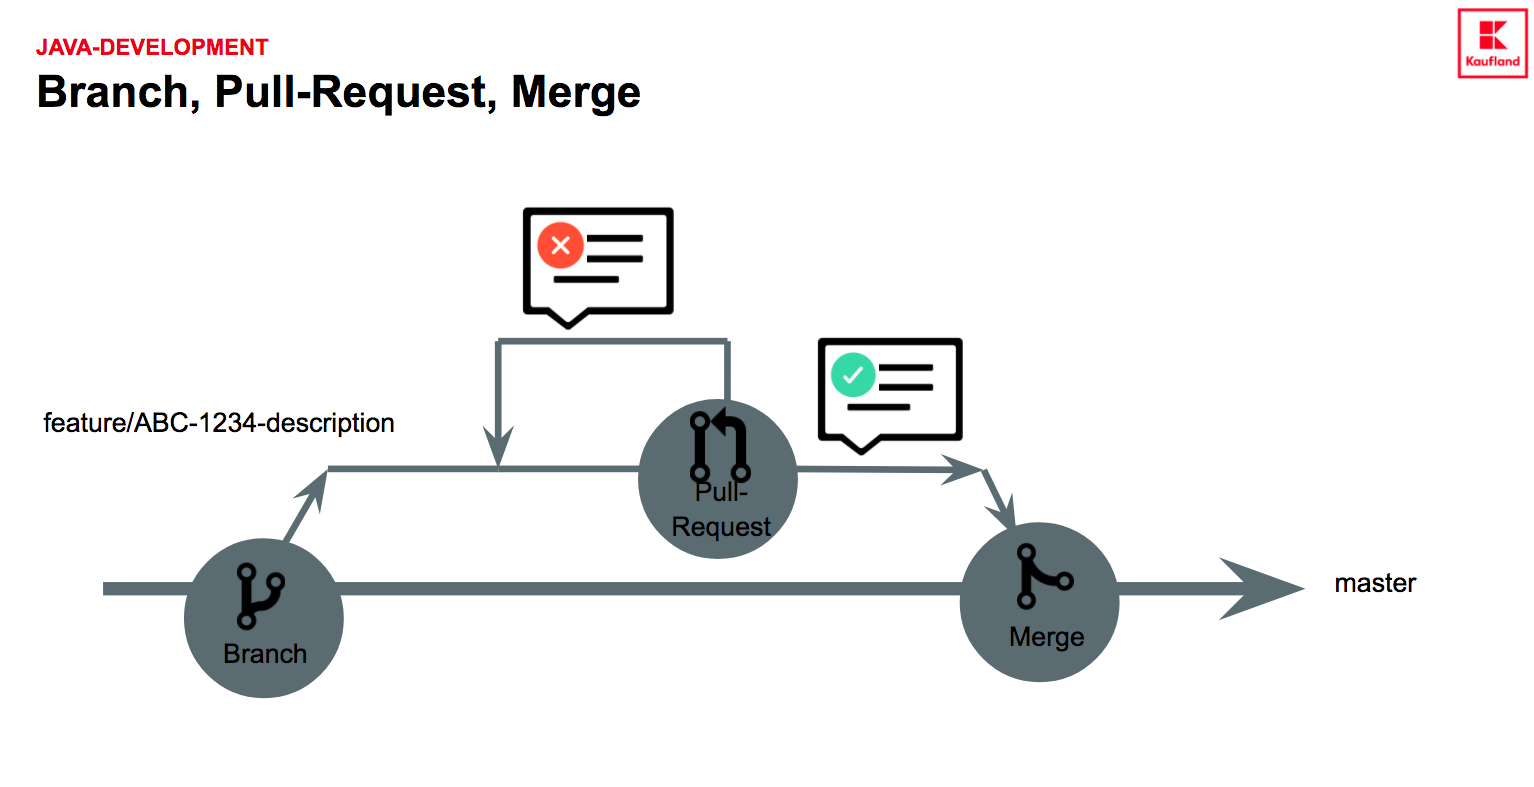
\includegraphics[width=\textwidth]{include/images/Branch.png}
        \caption{Versionsverwaltung und Review}
        \label{fig-Versionsverwaltung}
    \end{figure}

    Damit die aktuell noch laufenden Prozesse nicht gestört werden, erstellt der Entwickler einen "Branch" in dem er seinen Code schreibt. Wenn er fertig damit ist testet er und wenn er keine Mängel feststellt, stellt er ein Pull-Request. Dann müssen mindestens zwei weitere Entwickler den Code "reviewen" und mit dem Code zufrieden sein damit er den "Branch" wieder "mergen" kann, also den von ihm geschriebenen Code wieder in den "masterbranch" (Hauptprogramm) einfügen kann. Dann trifft man sich wieder zu einem gemeinsamen Meeting zwischen FB, AE und BC und lässt das ganze Programm testen und der FB teilt mit ob seinen Vorstellungen entsprochen hat oder ob noch etwas geändert werden muss. Dann startet wieder der nächste Lauf mit der nächsten Idee.

    Alternativ kann man den Ablauf, nur auf den Entwickler fokussiert, so betrachten:

    \begin{figure}[H]
        \centering
        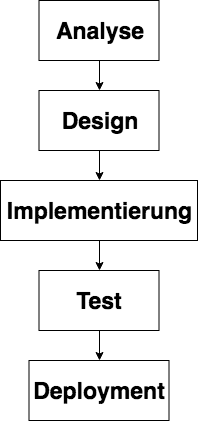
\includegraphics[width=5cm]{include/images/Arbeitsweise.png}
        \caption{Veeinfachte und auf den Entwickler bezogene Arbeitsweise}
        \small Man kann die Arbeit eines Entwicklers in 5 Abschnitte einteilen. Von einem späteren Abschnitt kann bei Fehlern oder ähnlichem auch wieder zu einem früheren zurück gekehrt werden.
        \label{fig-Arbeitsschema}
    \end{figure}

    Zuerst analysiert der AE das Problem, dann überlegt er sich wie er es lösen kann und schreibt diese Lösung als Code nieder. Den fertigen Code testet er auf Fehler, wenn keine vorhanden sind, ist seine Arbeit getan. 

\section{wichtige Fähigkeiten}

\begin{figure}[H]
    \centering
    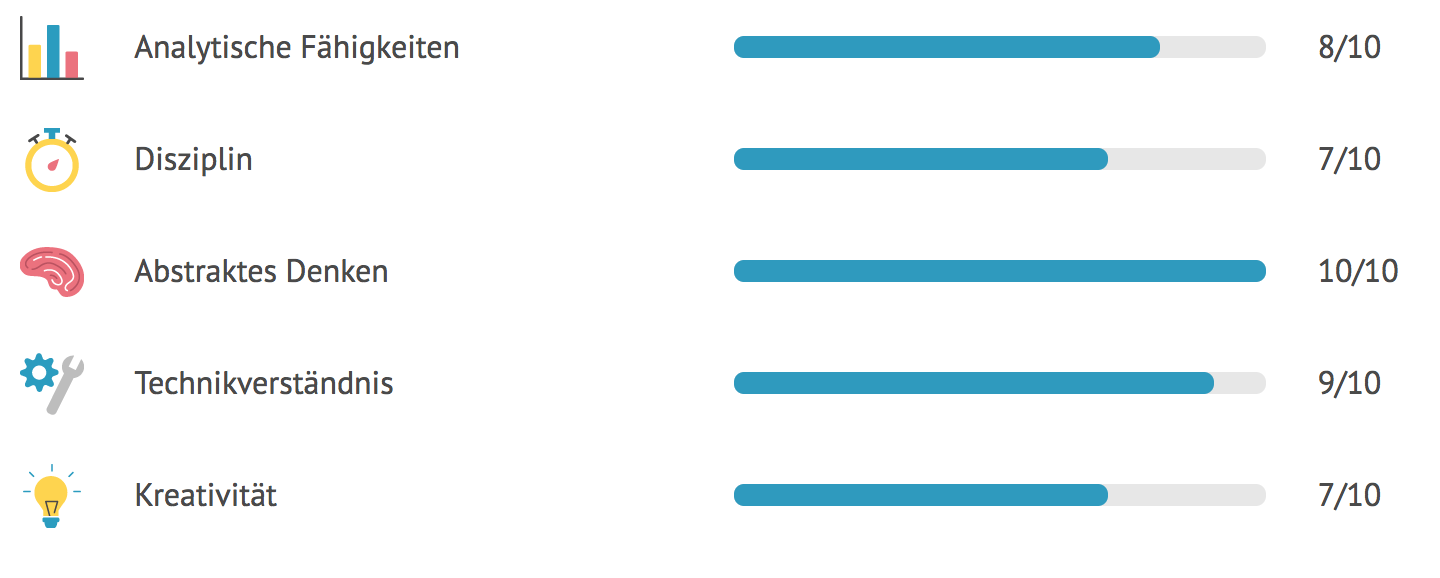
\includegraphics[width=\textwidth]{include/images/Faehigkeiten.png}
    \caption{Fähigkeiten eines AEs}
    \small Je mehr Punkte die jeweilige Fähigkeit erhält, desto wichtiger ist sie.
    \label{fig-Faehigkeiten}
\end{figure}

Wie in diesem Diagramm zu erkennen, sind abstraktes Denken, Technikverständnis und analytische Fähigkeiten am wichtigsten. Aber auch soziale Kompetenzen, wie z. B Teamfähigkeit sind gerade beim gemeinsamen entwickeln oder kommunikative Fähigkeiten bei den Besprechungen, sind gefragt. Lange still sitzen zu können ist auch wichtig. Wenn wichtige Systeme ausfallen muss man allerdings auch unter Druck arbeiten können um die Störung schnellstmöglich zu beheben. Da nicht die Zeit vorhanden ist um alle Dinge beigebracht zu bekommen, sind auch autodidaktische Fähigkeiten von Nöten. Für den Anfang sind aber vor allem die Abschlussnoten des Studiums ausschlaggebend. 

\section{Umgang mit dem Arbeitsumfeld}

    Als AE muss man vor allem für seine eigene Arbeit Verantwortung übernehmen. Als Führungskraft natürlich auch für seine Mitarbeiter. Eigeninitiative kann man dann zeigen, wenn man selbst ein Problem in einem System entdeckt oder ein Optimierungsvorschlag einbringt. 

\section{Zukunftsprognose}

In Zukunft werden sehr wahrscheinlich immer mehr AEs gebraucht, da in jeder Branche immer mehr automatisiert wird und um die dafür verwendeten Prozesse zu optimieren und überhaupt zu entwickeln werden immer mehr AEs benötigt. Auch momentan wird akribisch nach guten AEs gesucht. 